The system can be configured using the GUI. Available configuration settings is checkpoint circles, door mask area, exclusion mask and grayscale height threshold settings. 

The circles should be placed so persons walking into the room inevitable will pass all three lines. They should also be more inside the room compared to the door mask area. A good placement is illustrated in figure \ref{fig:circlePlacement}. Note that the red, most inner circle, includes the upper corners of the door frame. A too small inner circle will cause people to miss it and will therefore not be detected. 

\begin{figure}[H]
	\centering
	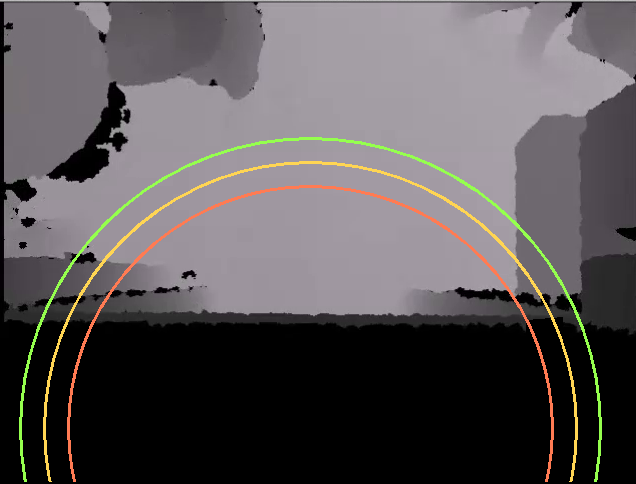
\includegraphics[width=\linewidth]{images/Manual2.png}
	\caption[Circle placment]{\textit{A prefered placement of the circles. }}
	\label{fig:circlePlacement}  %Skapar referens till figuren
\end{figure}

\newpage
The door mask should cover the area close to the door where people appear. It is important to make this area big enough, rather too big than too small. It can, but should not cover the upper, most distant, part of the red circle, figure \ref{fig:doorMask} illustrates this.

\begin{figure}[H]
	\centering
	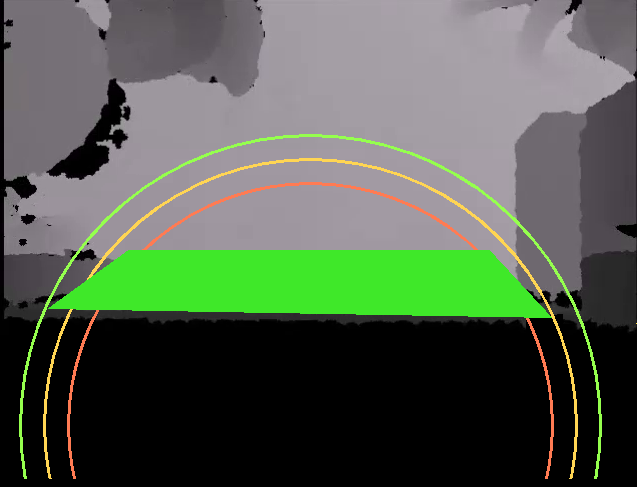
\includegraphics[width=\linewidth]{images/Manual3.png}
	\caption[Exclusion mask]{\textit{The prefered placement of the door mask, the door mask is the green area.}}
	\label{fig:doorMask}  %Skapar referens till figuren
\end{figure}

\newpage
Exclusion masks should cover areas where people can not walk or appear. This could be areas like tables or areas behind the door (walls in this case), figure \ref{fig:exMask} illustrates this. Note that for long usage of the system, movable furniture should not be excluded.

\begin{figure}[H]
	\centering
	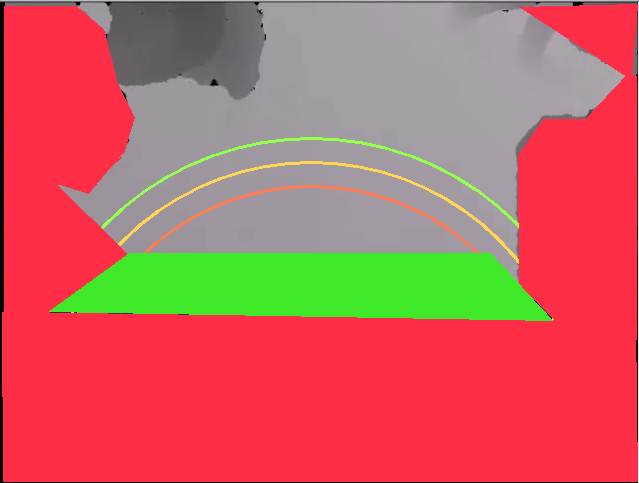
\includegraphics[width=\linewidth]{images/Manual1.png}
	\caption[Exclusion mask]{\textit{Exclusion mask is marked as red. It covers areas where people can not walk or appear.}}
	\label{fig:exMask}  %Skapar referens till figuren
\end{figure}


\newpage
\subsection{Config file}
The config file used by the algorithm pipeline is called \textit{dense\_conf.yml}. In it any configurable variable in any algorithm currently selected to be in the pipeline can be specified. The pipeline itself can also be specified, allowing fo rapid swapping of algorithms. The most useful variables in the current pipeline are shown in table \ref{table:commonVariables}.\\

\begin{table}[hbt]
	\begin{tabular}{ | l | l | p{7.5cm} | }
	    \hline
	    \textbf{Variable} & \textbf{Algorithm/Program-part} & \textbf{Description} \\ \hline
	    runFromFile & Network & If set to 1, the video sources are files found in the paths \textit{videoFilePaths}.  \\ \hline
	    videoFilePaths & Network & The paths to the video files used if running from file.  \\ \hline
	    useKinect & Network & If set to 1, the video sources are from Microsof Kinect cameras. \\ \hline
	    TrackingMaximumDistance & Tracking & The maximum distance an object can be considered to have moved since last frame. \\ \hline
	    TrackingMinimzumLifeSpan & Tracking & The minimal time (in \# frames) a potential object must have existed (and been tracked) before it is considered a real object. \\ \hline
	    TrackingMaximumTimeLost & Tracking & The maximum time (in \# frames) an object is allowed to be lost before it is forgotten. \\ \hline
	    lowestDistanceOverFloor & Kinect Segmentation & The limit (height units) of how short a person can be. Set this variable using the GUI calibration utility described previously. \\ \hline
	    webServerUrl & Network & The address to the web service to which results are reported. \\ \hline
	\end{tabular}
	\label{table:commonVariables}
	\caption{The most useful and common variables in the current pipeline.}
\end{table}

\newpage
Currently the pipeline consists of two major algorithms: \textit{ImageProcessor} and \textit{Analytics}. These in turn have several sub-algorithms that are executed in the order specified in the config file. The current pipeline is structured in the following way: \\
\hspace*{0.5cm}\textit{ImageProcessor:\\
\hspace*{1cm}- KinectSegmentation\\
\hspace*{1cm}- TrackingBruteForce}\\
\hspace*{0.5cm}\textit{Analytics:\\
\hspace*{1cm}- EntryExitCounter\\
\hspace*{1cm}- FlowEstimator\\
\hspace*{1cm}- QueDetector\\
\hspace*{1cm}- QueSeverityEstimator}\\\\
Any algorithm registed in the system can be used as a subalgorithm for any other algorithm, writing in the config file in the same way as with \textit{KinectSegmentation} being a sub algorithm to \textit{ImageProcessor}. To get an empty algorithm placeholder any none-registerd algorithm name (or variable name) may be used, such as:\\
\hspace*{0.5cm}\textit{UnregisterdName:\\
\hspace*{1cm}- KinectSegmentation\\
\hspace*{1cm}- ...}\\
It can now be used as a sub-algorithm to another algorithm (or placeholder algorithm):\\
\hspace*{0.5cm}\textit{ImageProcessors:\\
\hspace*{1cm}- UnregisterdName\\
\hspace*{1cm}- ...}\\
A placeholder algorithm works by just passing through initialization and processing calls to its sub-algorithms.\\\\
\textbf{Warning: If you do not know what your are doing, do not modify the algorithm pipeline. Some algorithms have requirements which must be provided by earlier algorithms, the system will not run if these are not met. See the code documentation for further details on requirements and effetcs of different algorithms.}

